\documentclass{icmmcm}

\usepackage{url}
\usepackage{graphicx}
%\usepackage{listings}

\newcommand{\der}{\mathrm{d}}

\title{A Research of Something}
\team{38403}
\question{A}
\date{February 8, 2015}

\begin{document}
\begin{summary}
Summary
\end{summary}

\section{Model}
\subsection{The Spread of the Ebola Virus}
For convenience, we defined some symbols:
\begin{center}
\begin{tabular}{|r|p{7cm}|}
\hline
$ i(t) $ & total cases on $t$-th day.\\
\hline
$ i(0)=i_0 $ & total cases on beginning.\\
\hline
$ N $ & population in this area.\\
\hline
$ k $ & infect factor\\
\hline
$ r(t) $ & number of people exited from the epidemic process on
$t$-th day.\\
\hline
%$ p_0 $ & \\
%\hline
\end{tabular}
\end{center}%
\textbf{\large Modeling:}\\
\textbf{Case 1:}\\
Assumptions:
\begin{enumerate}
  \item There is no body recover or die in the present period.
  \item Population $ N $ remain unchanged, it means
  that we don't care population death,birth and flow.
  \item Take $ k_0 $ as the number of people infected by
a patient in one day.
%  \item The ebola virus no variation in the present period.
\end{enumerate}
The increasement of cases from $ t $ to $ t+\Delta t$ is:
\begin{equation}
i(t+\Delta{t})-i(t)=k_0i(t)\Delta{t}
\label{equ:1}
\end{equation}
we can get a ordinary differential equations model for 
equation (\ref{equ:1}):
\begin{equation}
\left\{
\begin{array}{l}
\frac{{\der}i(t)}{{\der}t}=k_0i(t)\\
i(0)=i_0
\end{array}\right.
\label{equ:2}
\end{equation}
the solution of equation (\ref{equ:2}) is:
\begin{equation}
i(t)=i_0e^{k_0t}
\label{equ:3}
\end{equation}
the figure of equation (\ref{equ:3}) is figure~\ref{fig:1}:\par
\begin{figure}
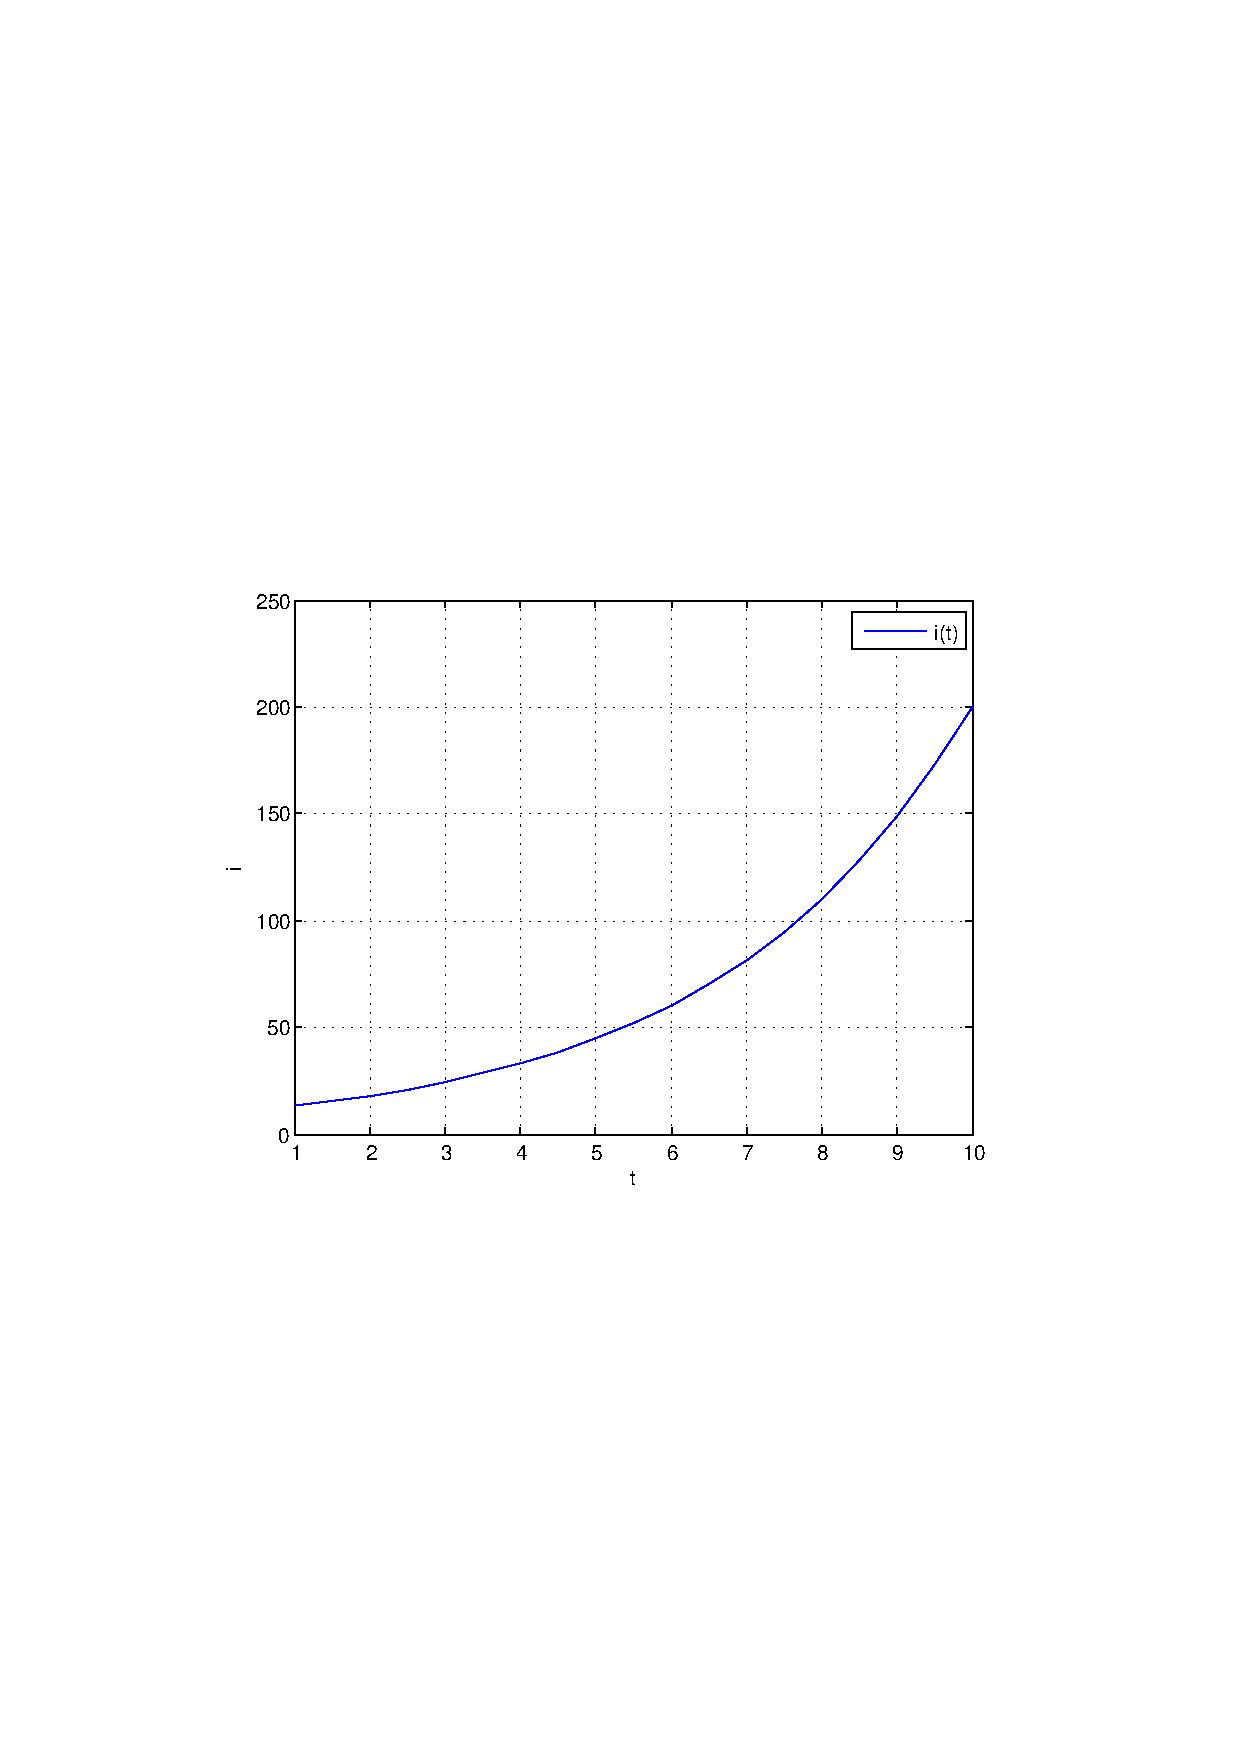
\includegraphics[width=4in]{imgs/i(t).pdf}
\caption{equation (\ref{equ:3})}
\label{fig:1}
\end{figure}
the figure~\ref{fig:1} shows us that: 
The Ebola virus spread increases exponentially.
The results are in good agreement with 
the Ebola virus spread in beginning, in general, Ebola
spread speedy in beginning, the infected person growth in the
exponential function, when $t$ tends to infinity, then $i(t)$
tends to infinity. But the actual situation of the Ebola virus
late is not fit, because in the patients's effective
contact crowd, have healthy people and patients, while only
health personnel can be infected. And part of patients will die
in this period.\par
Improve this model, then we have case 2.\\
\textbf{Case 2:}\\
Assumptions:
\begin{enumerate}
  \item Assuming infected and cured with long-term immunity,
   does not consider the case of long-term repeated infections,
   healthy immediately after infection can become infected
   persons. In this case, the people of the entire region is
   divided into three categories: The first category is
   contagium which able to infect others, indicating
   the number of such moment $ t $ with $ i(t) $; second
   category is susceptible which vulnerable to becoming infected, 
   with $ s(t) $ represents the number of such moment $ t $;
   the third category is a person other than the two
   categories above, including death after infection,
   get a long-term immunity after illness, who are
   no longer infected, represents the number of such
   moments $ t $ with $ r(t) $.
  \item The region's total population $N$ remain unchanged
   during the discussion, that is not considered births, deaths,
   flow and so on.
  \item The speed of change from first class to second class is
   proportional to the number of first class.
\end{enumerate}
\begin{equation}
k=\frac{k_0}{s(t)}
\label{equ:4}
\end{equation}

\begin{equation}
l=\frac{\frac{{\der}r(t)}{{\der}t}}{i(t)}
\label{equ:5}
\end{equation}

\begin{equation}
\left\{
\begin{array}{l}
\frac{{\der}r(t)}{{\der}t}=li(t)\\
\frac{{\der}i(t)}{{\der}t}=ks(t)i(t)-\frac{{\der}r(t)}{{\der}t}\\
\frac{{\der}s}{{\der}t}=-\frac{{\der}i(t)}{{\der}t}-\frac{{\der}r(t)}{{\der}t}
\end{array}\right.
\label{equ:6}
\end{equation}

$ i(0)=i_0,s(0)=s_0,r(0)=r_0=N-i_0-s_0 $

\begin{equation}
\left\{
\begin{array}{l}
\frac{{\der}i(t)}{{\der}t}=ks(t)i(t)-li(t)\\
\frac{{\der}s(t)}{{\der}t}=-ks(t)i(t)\\
\frac{{\der}r(t)}{{\der}t}=li(t)\\
i(0)=i_0,s(0)=s_0,r(0)=r_0=N-i_0-s_0
\end{array}\right.
\label{equ:7}
\end{equation}
\begin{figure}
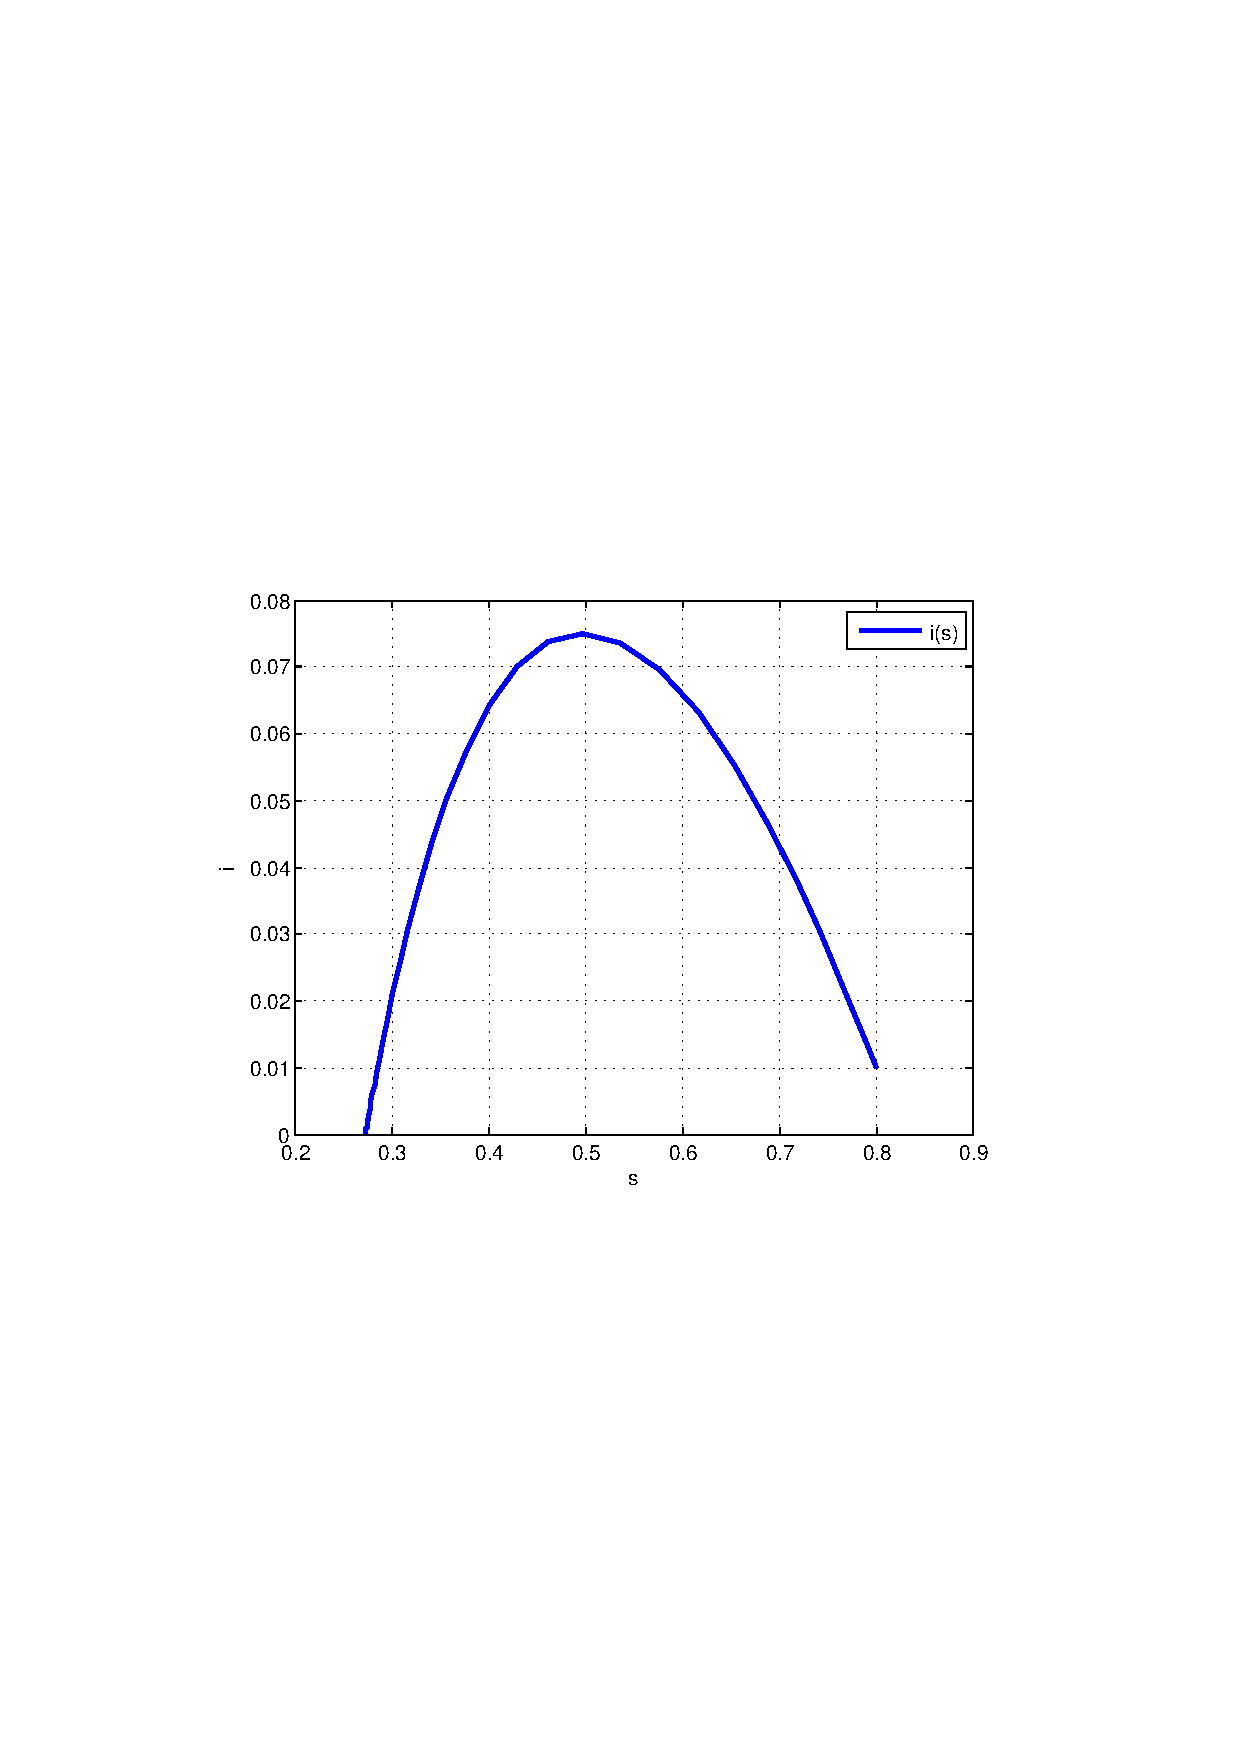
\includegraphics[width=4in]{imgs/sars3_2.pdf}
\caption{Phase trajectoriesthe for equation (\ref{equ:7})}
\label{fig:2}
\end{figure}
Equation (\ref{equ:7}) is difficult to obtain an accurate
solution can be the first to make numerical calculations.\par
Numerical Methods: For convenience of calculation, visual
 $ s(t) $ and $ i(t) $ is the proportion of the total number,
 and therefore, in equation (\ref{equ:7}), set $k=1$,
  $l=0.5$, $i(0)=0.01$, $s(0)=0.80$, using MATLAB software
 programming as appendix 1 and 2, product Figure~\ref{fig:2}
Elimination $ t $:
\begin{equation}
\frac{{\der}i}{{\der}s}=-1+\frac{1}{ks}
\label{equ:8}
\end{equation}
Set $\rho=1/k$, said $\rho$ is a characteristic (on the
same area and the same infectious,$\rho$ is a constant).
\begin{equation}
\frac{{\der}i}{{\der}s}=\frac{\rho}{s}-1
\label{equ:9}
\end{equation}

\begin{equation}
i(s)=\rho lN\frac{s}{s_0}-s+s_0+i_0
\label{equ:10}
\end{equation}

Draw its figure:\par
\begin{center}
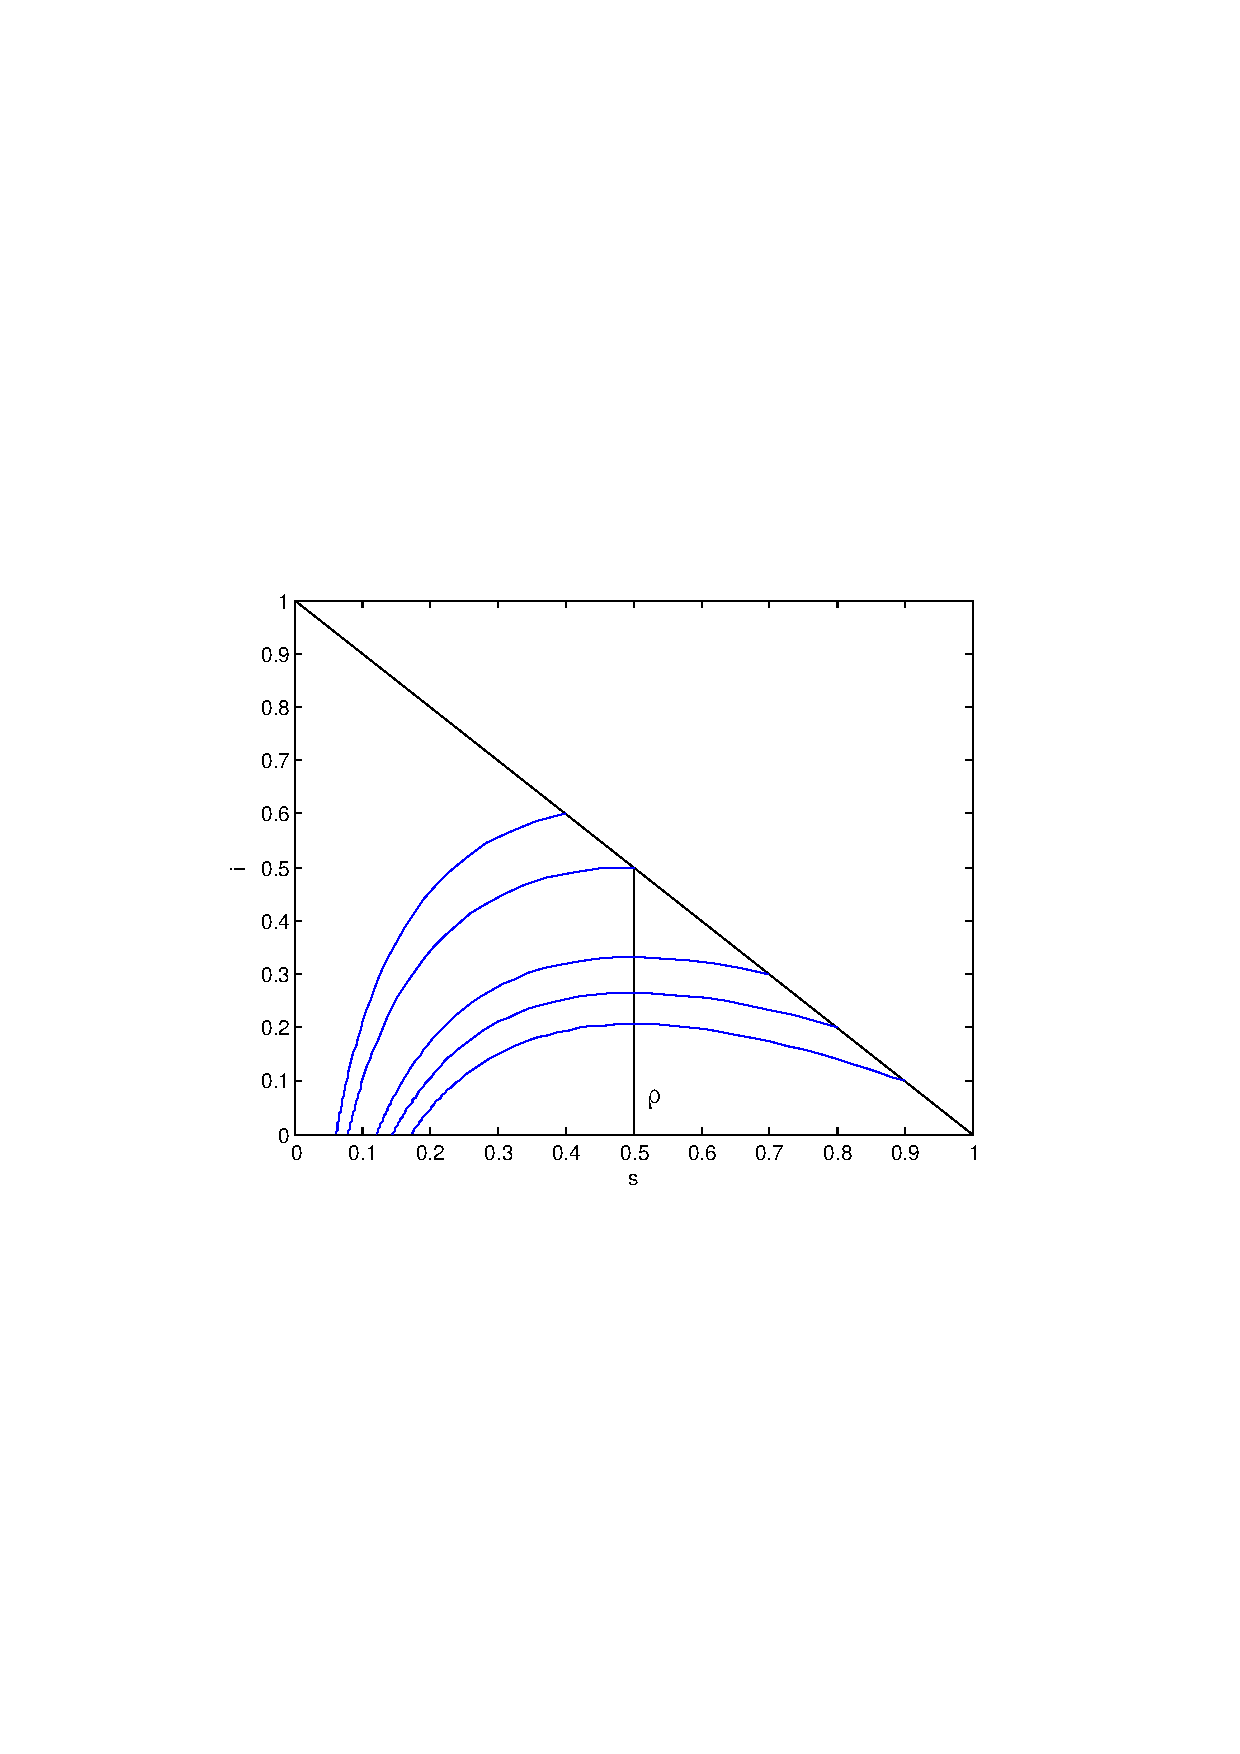
\includegraphics[width=4in]{imgs/i(s)_i_s.pdf}
\end{center}

From this figure, we can see that:
\begin{enumerate}
  \item regardless of where the phase trajectoriesthe start on,
   it will eventually intersect with the $s$ axis,
   that is the patient will eventually disappear;
  \item the final uninfected healthy proportion is
   $s_m$(when $t\rightarrow\infty$);
  \item if $s_0>\rho$, the $i(t)$ first increase, while when 
   $s=\rho$, $i(t)$ reaches a maximum:
   $$
	i_m=s_0+i_0-\rho(1+lN\frac{s_0}{\rho})
   \label{equ:11}
   $$
   Then, $i(t)$ decreases and tends to zero, $s(t)$ is
   monotonically reduced to $s_m$.
  \item If $s_0<\rho$ then $i(t)$ decreases monotonically to
   0, $s(t)$ decreases monotonically to $s_m$.
\end{enumerate}
The following study relationship between Ebola virus spread and
time of begin taking isolation.\par
The figure below is based on Figure~\ref{fig:2} with changeing
the time when start taken to isolate, when $l$ will increase.
Figure~\ref{fig:4}(B) is the effect of different time of begin taking 
isolation for the number of patient, $1,2,\cdots,n$ hour
corresponding image by the bottom-up.(MATLAB code for this part
is in appendix 1, 3 and 4)\par
\begin{figure}\centering
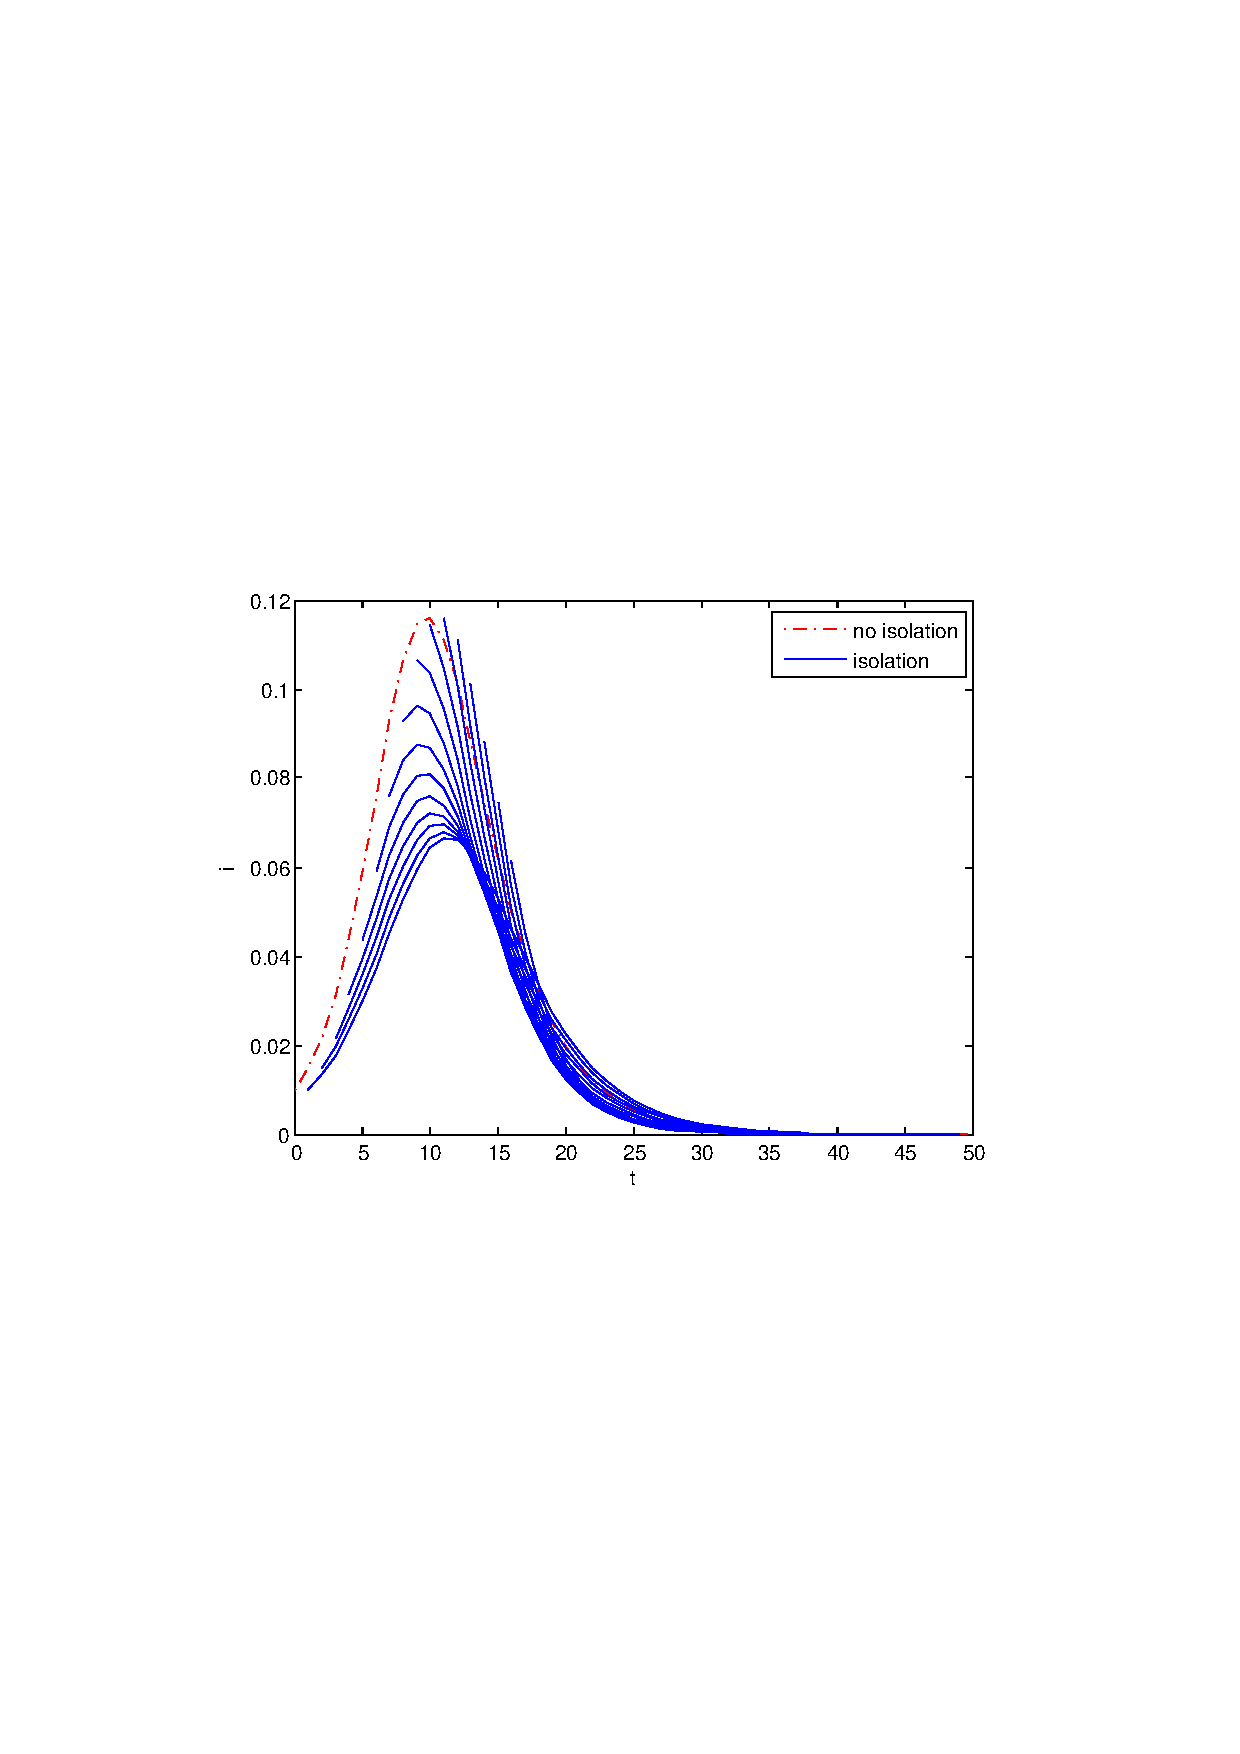
\includegraphics[width=4in]{imgs/iso_i_t.pdf}
\nline%
(A)
\\\nline%
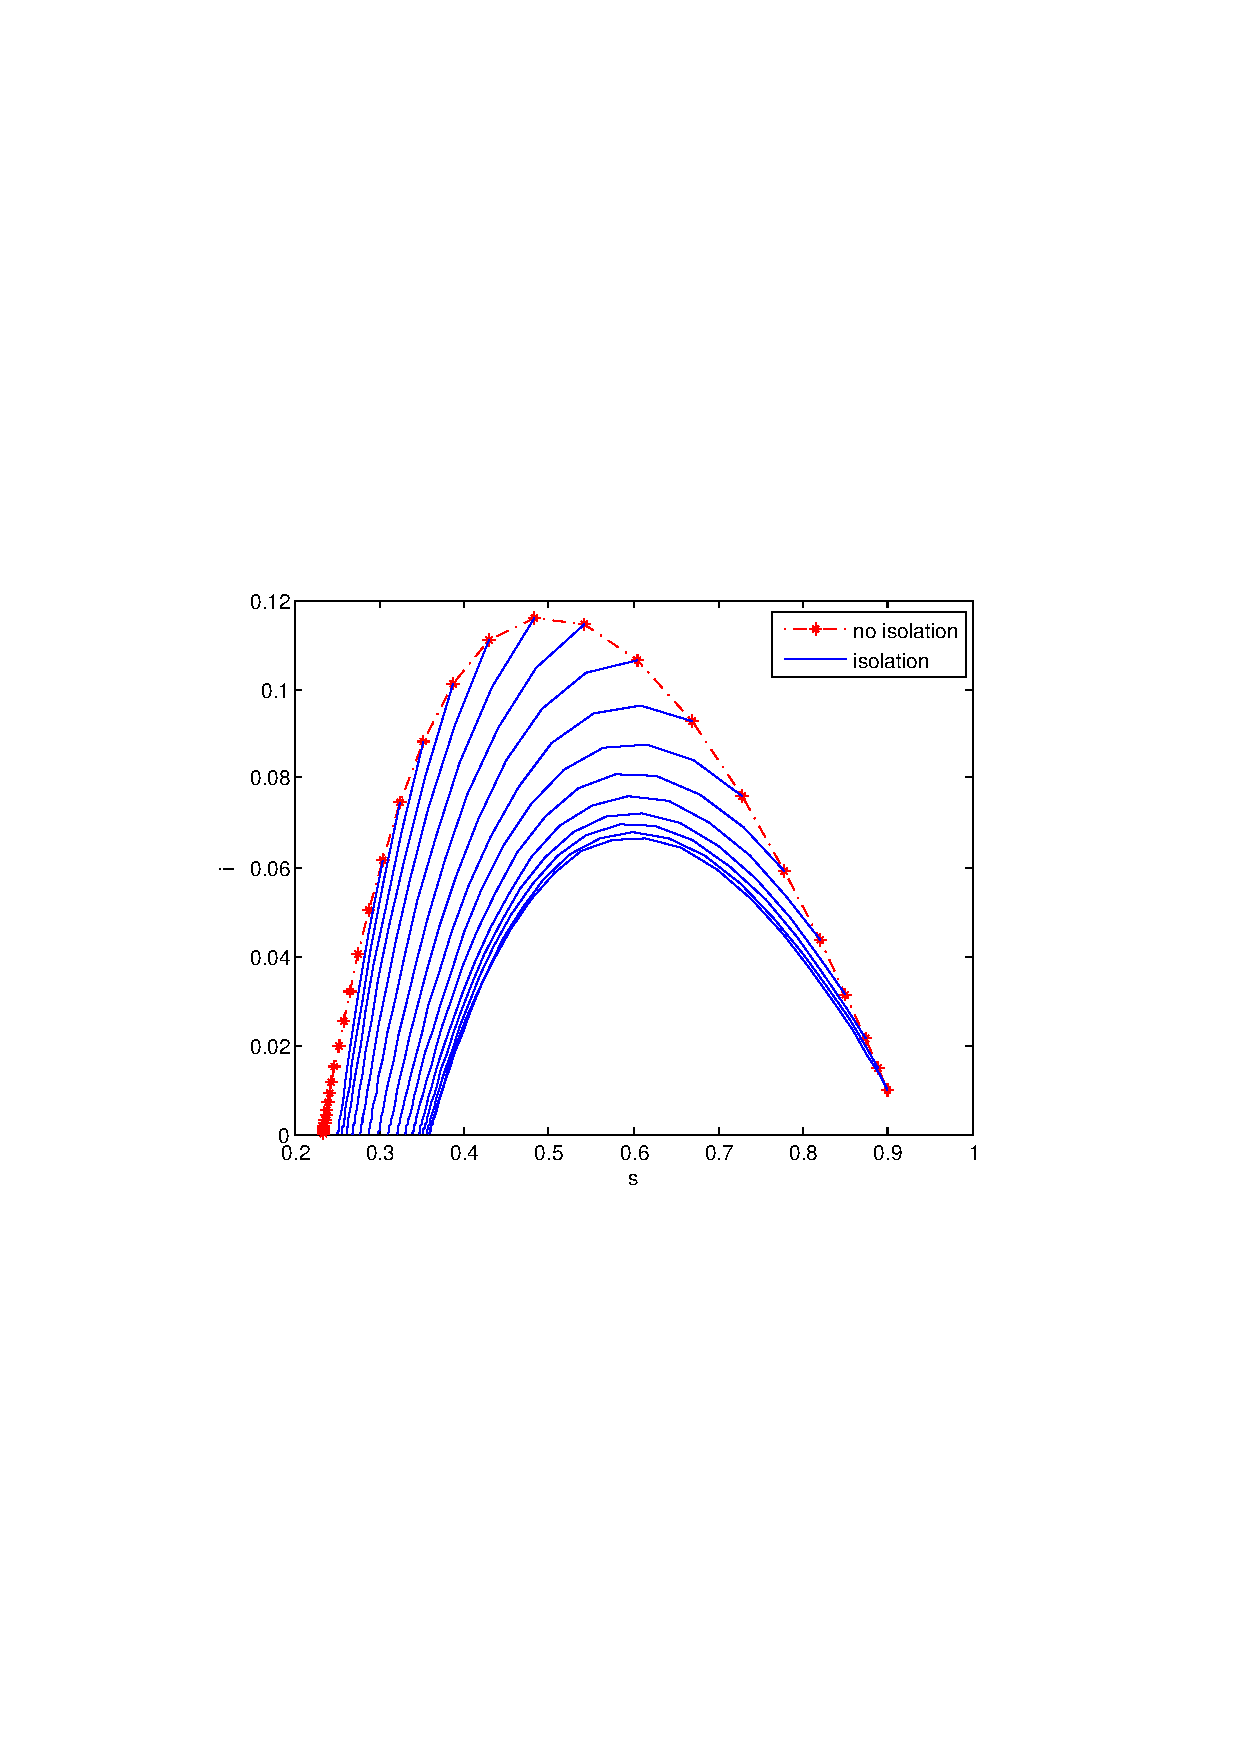
\includegraphics[width=4in]{imgs/iso_i_s.pdf}
\nline%
(B)
\caption{The effect of different time of begin taking 
isolation for spread.}
\label{fig:4}
\end{figure}
As can be seen from Figure~\ref{fig:4}(A), with the start of
the time taken to isolation increasing, from the dense
continuous curve becomes too sparse, that is, at the time of
virus infection, in a certain period of time, little change in
the number of infected, but in the longer time to take
isolation, the number of infections is growing rapidly.
As can be seen from Figure~\ref{fig:4}(B), when began to take
isolated relatively in short time , the maximum number of
infections is relatively small, but with a long time, the sharp
increase in the number of infections. So once found infected
should be isolated as soon as possible, in 4h hours of isolation
is ideal, relatively small number of infections infected by per
patient, but if it start take isolation than 11h, then the
consequences will not optimistic, each patient infect
a lot of people.



\subsection{Required Drug}
Symbol definition:
\begin{center}
\begin{tabular}{|r|p{8cm}|}
\hline
$ p_0 $ & In the cure range, the maximum dosage required to
cure each Ebola patient.\\
\hline
$ Q(t) $ & The amount of drug at time $t$.\\
\hline
\end{tabular}
\end{center}%
Assumptions:
\begin{enumerate}
  \item The Ebola virus has no variation in the present period.
\end{enumerate}
The amount of the drug required to $ Q(t)=p_0*i(t) $.\par
The figure for $ i(t) $ in Case 2 shown as below:
\begin{center}
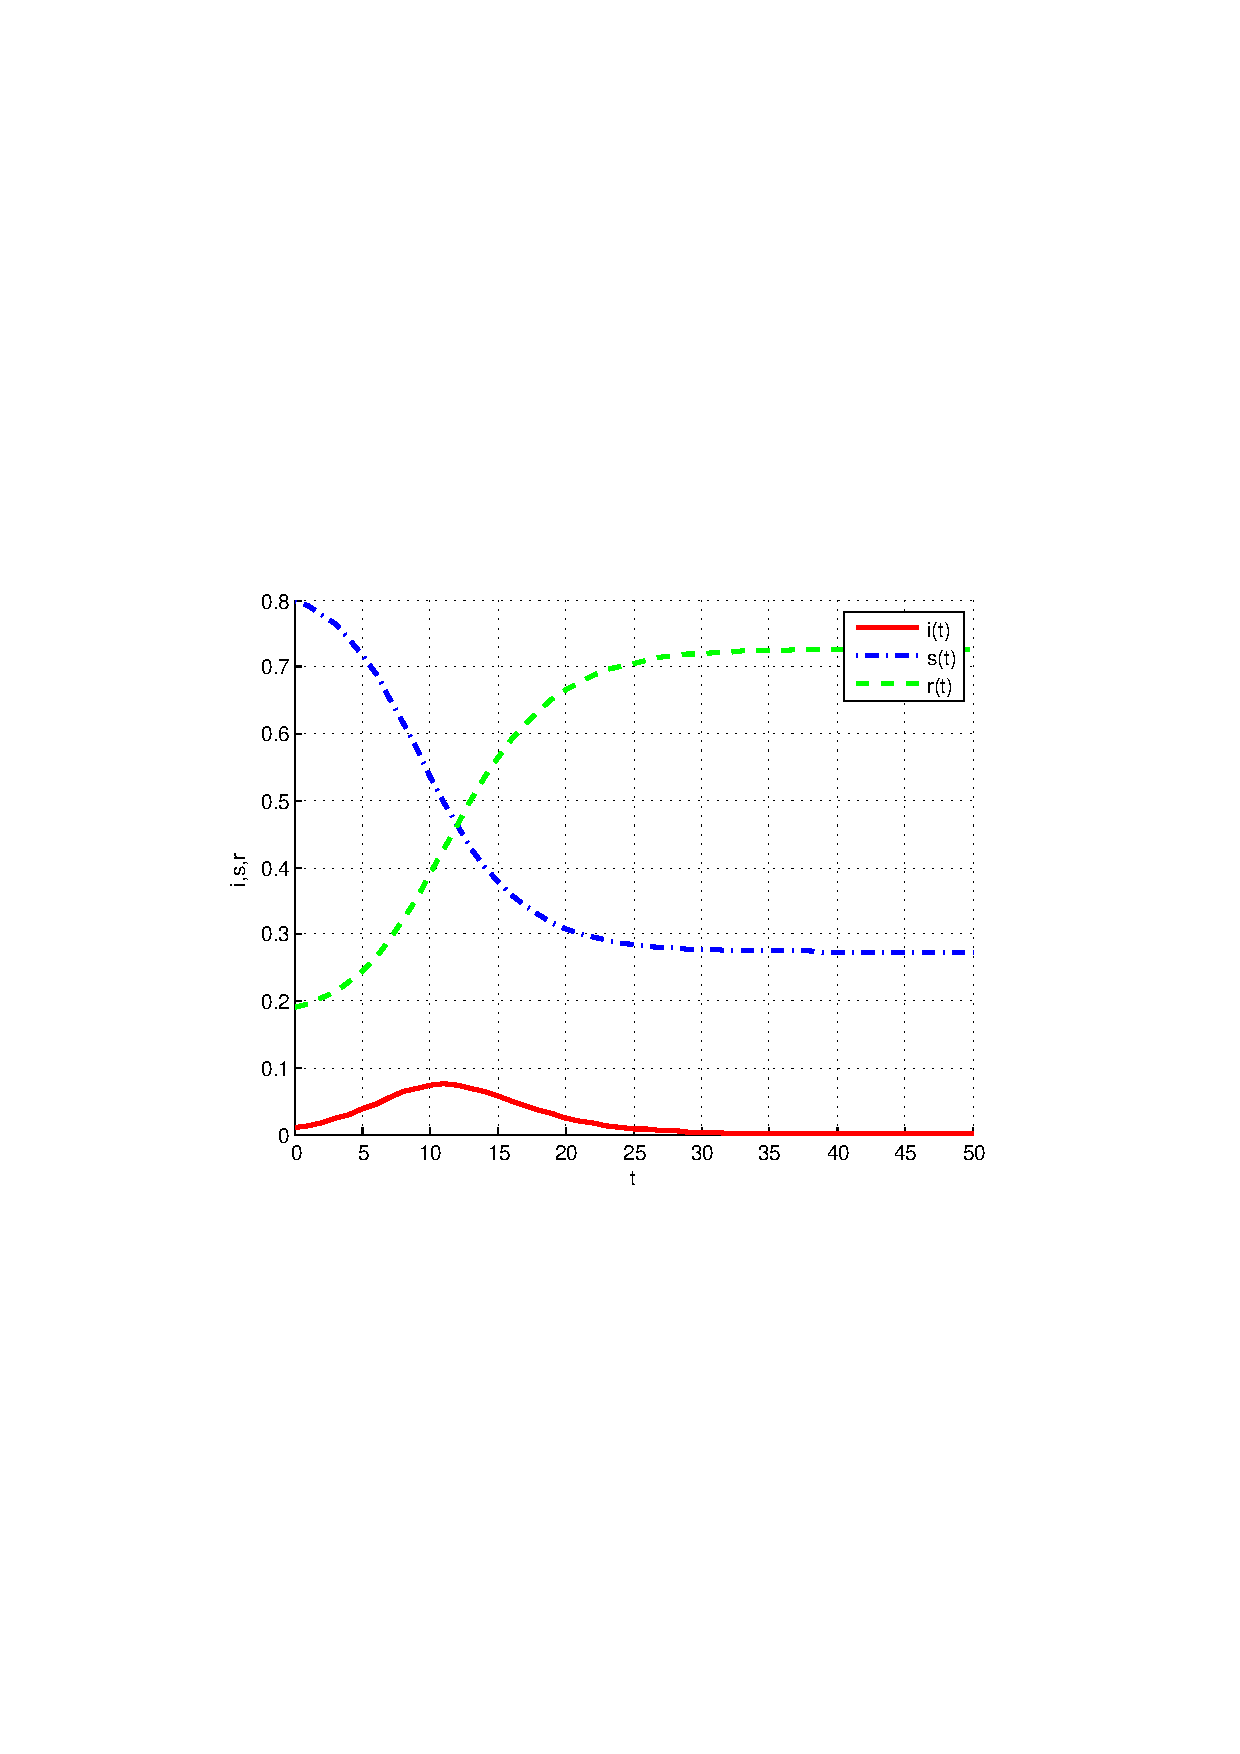
\includegraphics[width=4in]{imgs/sars3_1.pdf}
\end{center}
The amount of drug $Q(t)$ can be calculated is $p_0$ times of
$i(t)$, $Q(t)$ change with $t$ similar to $i$ change with $t$.

\subsection{Transportation System}
Symbol definition:
\begin{center}
\begin{tabular}{|r|p{8cm}|}
\hline
$ v(t) $ & The speed of the drug production at moment $t$.\\
\hline
$ v_0 $ & Transportation speed.\\
\hline
$ A_i $ & Drug production places.\\
\hline
$ B_j $ & Drug demanded place.\\
\hline
$ a_i $ & Producting speed of $A_i$.\\
\hline
$ b_j $ & Demand of $ B_j $.\\
\hline
$ x_{ij} $ & The quantity transport from $ A_i $ to
$ B_j $.\\
\hline
$ s_{ij} $ & the transportation path length from $A_i$ to $B_j$.\\
\hline
\multicolumn{2}{|c|}{$ i=1,2,\cdots,m;j=1,2,\cdots,n $}\\
\hline
\end{tabular}
\end{center}%
Assumptions:
\begin{enumerate}
  \item The number of patients increase with time in the short
term, to make patients whose illness is not serious can be
cured, the speed of the drugs production $ v(t) $ needs
increasing with time.
  \item Drug delivery using the same kind of transportation and
transportation speeds $ v_0 $ are consistent.
  \item There are $ m $ production places $ A_1,A_2,\cdots,A_m $
for the drug,the producting speed for the drug of $ A_i $ is
$ a_i $,$ i=1,2,\cdots,m $.There are $ n $ places $
B_1,B_2,\cdots,B_n $ need the drug,the demand of $ B_j $ is
$ b_j $,$ j=1,2,\cdots,n $.
  \item $ \sum_{i=1}^{m}a_i=\sum_{j=1}^{n} $.For all
$ i\in\{1,2,\cdots,m\} $ and $ j\in\{1,2,\cdots,n\} $, have
$ a_i,b_j>0 $.
% $ x_{ij} $ is the quantity of drug transported from $ A_i $ to
% $ B_j $,and $ s_{ij} $ is the transportation path length from
% $ A_i $ to $ B_j $.
\end{enumerate}
Modeling and solving:\\
Drug production time $ t=\frac{x_{ij}}{v(t)} $, drug
transportation time $ t'=\frac{s_{ij}}{v_0} $, let
$ c_{ij}=\frac{1}{v(t)} $, then:\\
\begin{equation}
\mathrm{min}~t''=\sum_{i=1}^{m}\sum_{j=1}^{n}(t+t')=
\sum_{i=1}^{m}\sum_{j=1}^{n}c_{ij}x_{ij} + 
\sum_{i=1}^{m}\sum_{j=1}^{n}t'
\label{equ:31}
\end{equation}
$$
s.t. \left\{
\begin{array}{l}
  \sum_{j=1}^{n}x_{ij}=a_i,i=1,2,\cdots,m \\
  \sum_{i=1}^{m}x_{ij}=b_j,j=1,2,\cdots,n \\
  x_{ij}\geq 0,i=1,2,\cdots,m, j=1,2,\cdots,n
\end{array}\right.
$$
where $ \sum_{i=1}^{m}\sum_{j=1}^{n}t' $ is certain, 
we just calculate the minimum of 
$ \sum_{i=1}^{m}\sum_{j=1}^{n}c_{ij}x_{ij} $.\\
Let:
$$
\begin{array}{ll}
x & = ~\begin{pmatrix}
	  x_{1,1} & x_{1,2} & \cdots & x_{1,n} \\
	  x_{2,1} & x_{2,2} & \cdots & x_{2,n} \\
	  \vdots  & \vdots  & \ddots & \vdots  \\
	  x_{m,1} & x_{m,2} & \cdots & x_{m,n}
	 \end{pmatrix}\\\\
C & = ~\begin{pmatrix}
	  c_{1,1} & c_{1,2} & \cdots & c_{1,n} \\
	  c_{2,1} & c_{2,2} & \cdots & c_{2,n} \\
	  \vdots  & \vdots  & \ddots & \vdots  \\
	  c_{m,1} & c_{m,2} & \cdots & c_{m,n}
	 \end{pmatrix}\\\\
b & = ~\begin{pmatrix}
	  a_1 & a_2 & \cdots & a_m & b_1 & b_2 & \cdots & b_n
	 \end{pmatrix}\\\\
A & = ~\begin{pmatrix}
	  a_{1,1} & a_{1,2} & \cdots & a_{1,n} \\
	  a_{2,1} & a_{2,2} & \cdots & a_{2,n} \\
	  \vdots  & \vdots  & \ddots & \vdots  \\
	  a_{m,1} & a_{m,2} & \cdots & a_{m,n}
	 \end{pmatrix}
\end{array}
$$
where $ a_{ij}=e_i+e_{m+j} $, $ e_{i} $ is a column vector with
$ m+n $ elements, and $i$-th element is 1, otherwise 0. Then we
have:
$$
\mathrm{min}~z=Cx
$$
$$
s.t. \left\{\begin{array}{r}
  Ax=b\\
  x\geq 0
\end{array}\right.
$$
when $ \sum_{j=1}^{n}x_{ij}=a_i $, we can ensure the
availability of drugs in different place.

\section{Appendix}
\textbf{1.MATLAB code for function ill (ill.m):}
\begin{lstlisting}[language=Matlab]
function y = ill(t,x)
k=1;l=0.5;
y=[k*x(1)*x(2)-l*x(1);-k*x(1)*x(2)];
end
\end{lstlisting}\nline%
%
\textbf{2.MATLAB code for solve ill (sill.m):}
\begin{lstlisting}[language=Matlab]
ts=0:50;
x0=[0.01;0.80]
[t,x]=ode45('ill',ts,x0);[t,x]
figure(1);
clf;
hold on;
plot(t,x(:,1),'-r','LineWidth',2);
plot(t,x(:,2),'-.b','LineWidth',2);
plot(t,1-x(:,1)-x(:,2),'--g','LineWidth',2);
xlabel('t');ylabel('i,s,r');
legend('i(t)','s(t)','r(t)');grid on;%pause
figure(2);
plot(x(:,2),x(:,1),'LineWidth',2);
xlabel('s');ylabel('i');
legend('i(s)');
grid on;
hold off;
\end{lstlisting}\nline%
%
\textbf{3.MATLAB code for function ill2 (ill2.m) when taken
isolution:} \begin{lstlisting}[language=Matlab]
function y = ill2(t,x)
k=1;l=0.6;
y=[k*x(1)*x(2)-l*x(1);-k*x(1)*x(2)];
end
\end{lstlisting}\nline%
%
\textbf{4.MATLAB code for study the effect of different time of
begin taking isolation for spread:}
\begin{lstlisting}[language=Matlab]
dur=50;
ts=0:dur;
x0=[0.01;0.90];
figure(1);
[t,x]=ode45('ill',ts,x0);
plot(t,x(:,1),'r-.');
xlabel('t');ylabel('i');
hold on;
figure(2);
clf;
plot(x(:,2),x(:,1),'r*-.');
hold on;
for g=1:(dur/3)
    [t,xx]=ode45('ill2',ts((g+1):dur),x(g,:));
    figure(1);
    plot(t,xx(:,1));
    figure(2);
    plot(xx(:,2),xx(:,1));
end
xlabel('s');ylabel('i');
legend('no isolation','isolation');
hold off;
figure(1);
legend('no isolation','isolation');
hold off;
\end{lstlisting}\nline%
%

\maketitle
\thispagestyle{fancy}
\tableofcontents

%%% Uncomment the following lines if you have figures or tables in
%%% your report:
%% \listoffigures
%% \listoftables

\section{Introduction}
MCM is very difficult!\\
MCM is very difficult!\\
MCM is very difficult!\\
MCM is very difficult!\\
MCM is very difficult!
\begin{table}
\centering
\begin{tabular}{|l|l|}
\hline
table & test\\
\hline
Hello & world\\
\hline
\end{tabular}
\caption{Table test}
\label{tab:1}
\end{table}
\newpage
\section{Modeling}
MCM is very difficult!

\subsection{Subtitle}
Plain text.H

\subsection{Another subtitle}
More plain text.

\section{Conclusion}
Balabala\ldots

\bibliographystyle{plain}
\begin{thebibliography}{2}
\bibitem{bib1}Chidansh Amitkumar Bhatt, Mohan S. Kankanhalli,
Multimedia data mining: state of the art and challenges,
\url{http://link.springer.com/article/10.1007/s11042-010-0645-5}

\bibitem{bib2}F. Giannotti, D. Pedreschi, A. Pentland, P.
Lukowicz, D. Kossmann, J.
Crowley, D. Helbing,
A planetary nervous system for social mining and collective awareness,
\url{http://link.springer.com/article/10.1140/epjst/e2012-01688-9}

\end{thebibliography}

\end{document}
